\documentclass[tikz,border=10pt]{standalone}
\usepackage{tikz}
\usetikzlibrary{positioning,shapes,arrows.meta,calc,fit,backgrounds}

\begin{document}
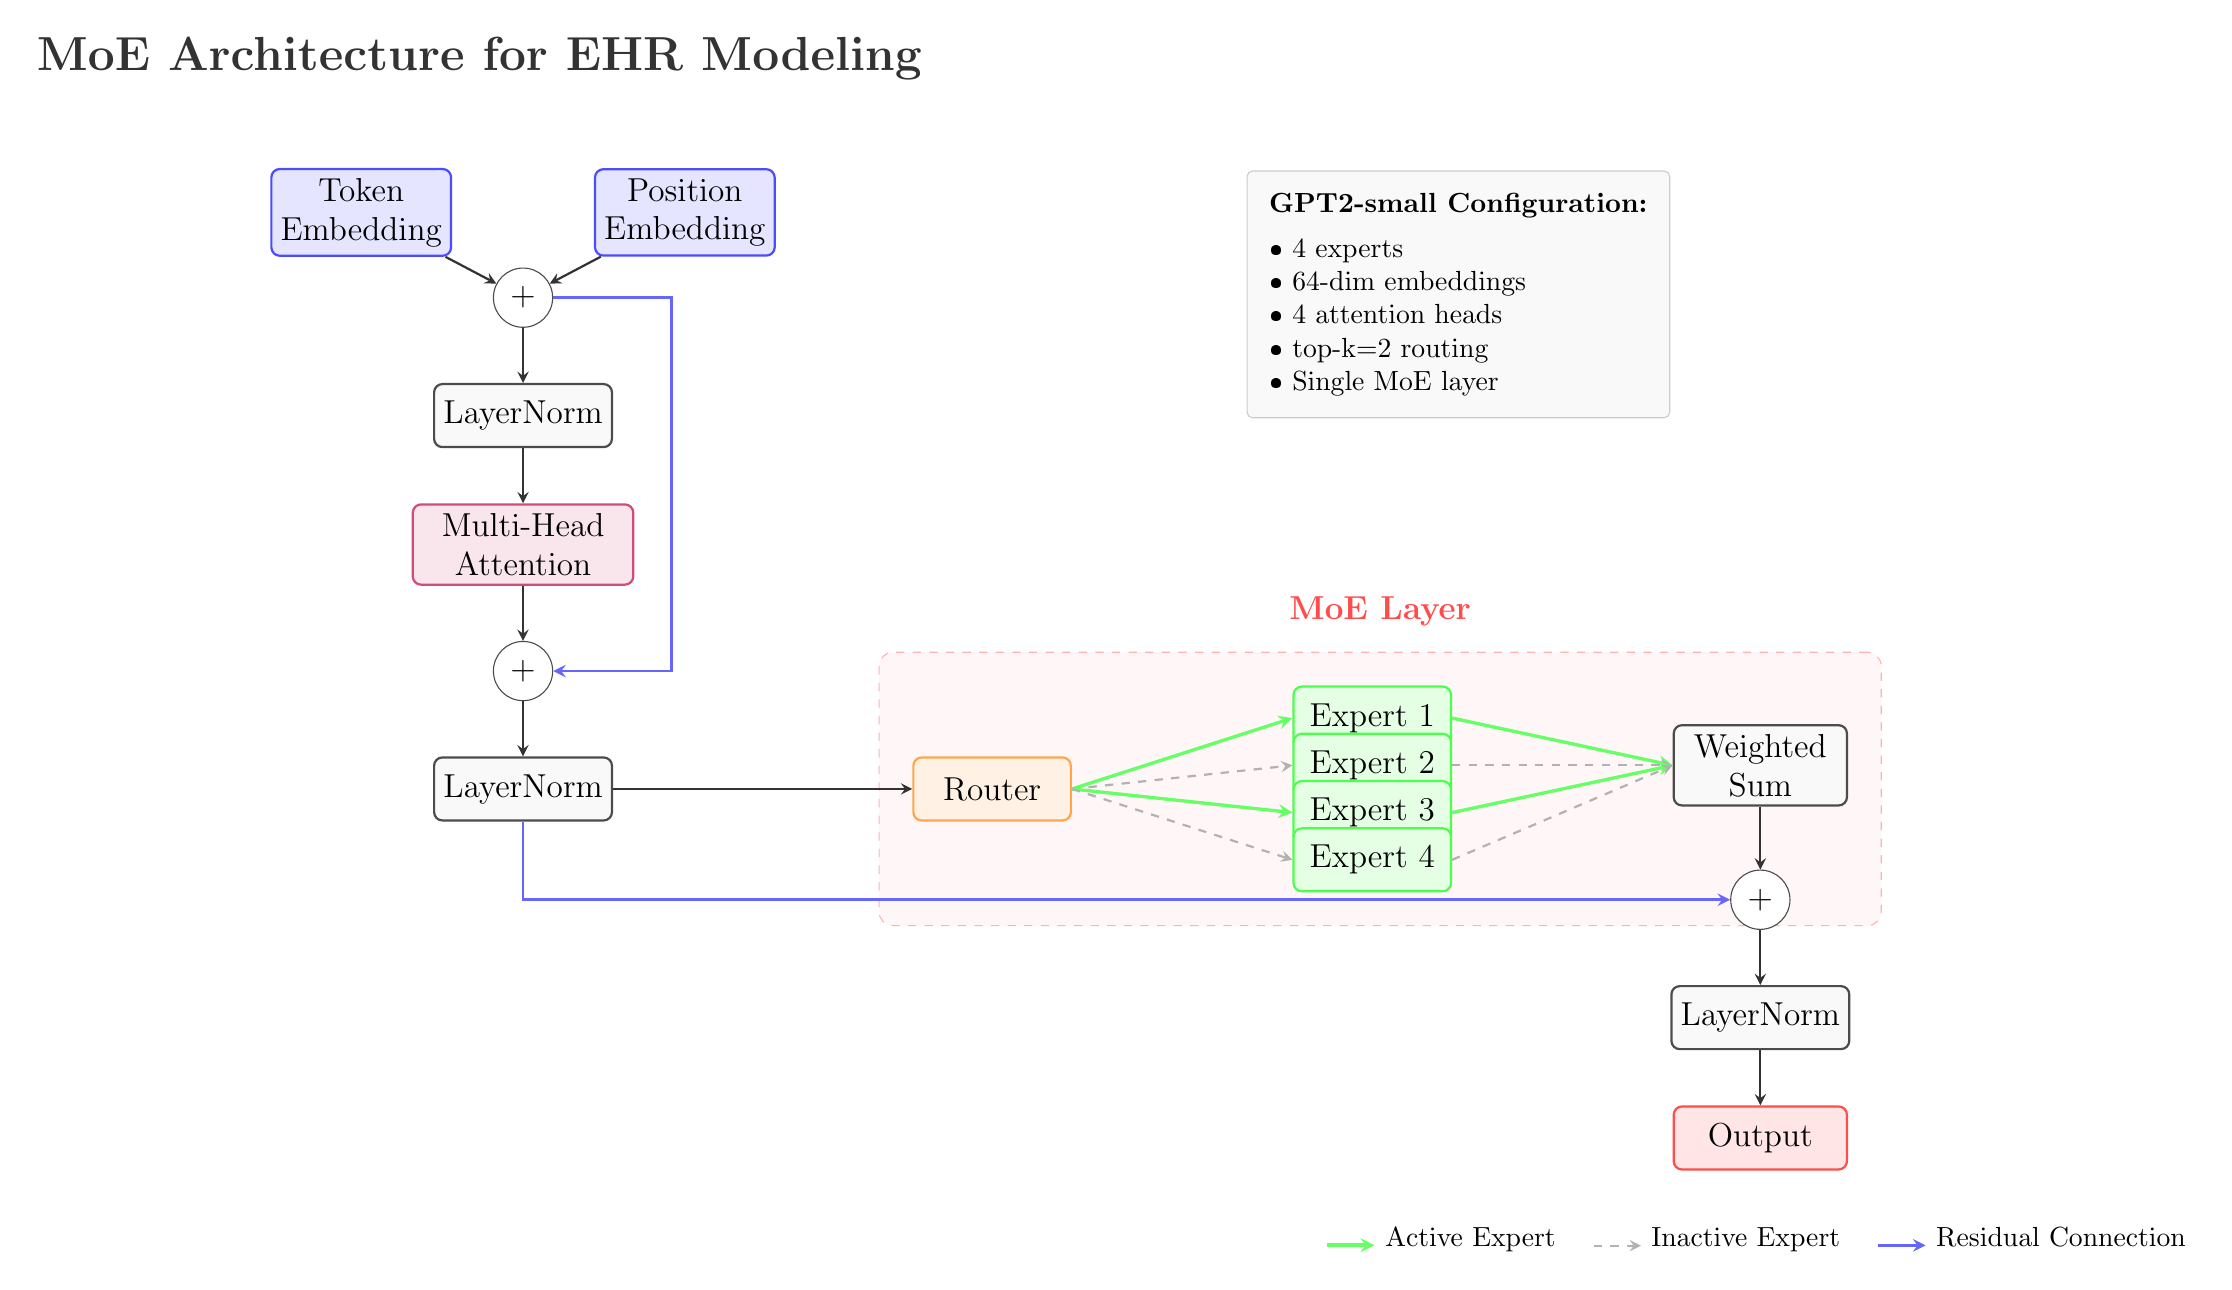
\begin{tikzpicture}[
    % Professional monochrome color scheme
    box/.style={rectangle, draw=black!70, fill=gray!5, rounded corners=3pt,
                minimum width=2.2cm, minimum height=0.8cm, align=center,
                font=\large, thick},
    embed/.style={box, fill=blue!10, draw=blue!70},
    attn/.style={box, fill=purple!10, draw=purple!70, minimum width=2.8cm},
    expert/.style={box, fill=green!10, draw=green!70, minimum width=2cm},
    router/.style={box, fill=orange!10, draw=orange!70, minimum width=2cm},
    output/.style={box, fill=red!10, draw=red!70},
    % Clean arrows
    arrow/.style={->, >=stealth, thick, black!80},
    active/.style={->, >=stealth, thick, green!60, line width=1.2pt},
    inactive/.style={->, >=stealth, thick, gray!60, dashed, line width=0.8pt},
    residual/.style={->, >=stealth, thick, blue!60, line width=1pt},
    node distance=0.8cm and 2.8cm
]

% Title - more prominent
\node[font=\LARGE\bfseries, color=black!80] (title) {MoE Architecture for EHR Modeling};

% Configuration box - better positioned and styled
\node[right=4cm of title, yshift=-3cm, align=left, font=\normalsize, 
      draw=gray!40, fill=gray!5, rounded corners=2pt, inner sep=8pt] (config) {
    \textbf{GPT2-small Configuration:}\\[0.15cm]
    • 4 experts\\
    • 64-dim embeddings\\
    • 4 attention heads\\
    • top-k=2 routing\\
    • Single MoE layer
};

% Input layer - better balanced
\node[embed, below=1.0cm of title, xshift=-1.5cm] (token) {Token\\Embedding};
\node[embed, right=1.8cm of token] (pos) {Position\\Embedding};
\node[circle, draw=black!70, fill=white, minimum size=0.6cm, 
      below=0.7cm of $(token)!0.5!(pos)$, font=\large] (add1) {+};

% Transformer stack - consistent spacing
\node[box, below=0.7cm of add1] (ln1) {LayerNorm};
\node[attn, below=0.7cm of ln1] (mha) {Multi-Head\\Attention};
\node[circle, draw=black!70, fill=white, minimum size=0.6cm, 
      below=0.7cm of mha, font=\large] (add2) {+};
\node[box, below=0.7cm of add2] (ln2) {LayerNorm};

% MoE section - better proportioned
\node[router, right=3.8cm of ln2] (gate) {Router};
\node[expert, right=2.8cm of gate, yshift=0.9cm] (exp1) {Expert 1};
\node[expert, right=2.8cm of gate, yshift=0.3cm] (exp2) {Expert 2};
\node[expert, right=2.8cm of gate, yshift=-0.3cm] (exp3) {Expert 3};
\node[expert, right=2.8cm of gate, yshift=-0.9cm] (exp4) {Expert 4};
\node[box, right=2.8cm of exp2, yshift=0cm] (sum) {Weighted\\Sum};

% Final layers
\node[circle, draw=black!70, fill=white, minimum size=0.6cm, 
      below=0.8cm of sum, font=\large] (add3) {+};
\node[box, below=0.7cm of add3] (ln3) {LayerNorm};
\node[output, below=0.7cm of ln3] (out) {Output};

% Main flow arrows - cleaner
\draw[arrow] (token) -- (add1);
\draw[arrow] (pos) -- (add1);
\draw[arrow] (add1) -- (ln1);
\draw[arrow] (ln1) -- (mha);
\draw[arrow] (mha) -- (add2);
\draw[arrow] (add2) -- (ln2);
\draw[arrow] (ln2) -- (gate);
\draw[arrow] (sum) -- (add3);
\draw[arrow] (add3) -- (ln3);
\draw[arrow] (ln3) -- (out);

% MoE routing - cleaner lines
\draw[active] (gate.east) -- (exp1.west);
\draw[inactive] (gate.east) -- (exp2.west);
\draw[active] (gate.east) -- (exp3.west);
\draw[inactive] (gate.east) -- (exp4.west);

\draw[active] (exp1.east) -- (sum.west);
\draw[inactive] (exp2.east) -- (sum.west);
\draw[active] (exp3.east) -- (sum.west);
\draw[inactive] (exp4.east) -- (sum.west);

% Cleaner residual connections
\draw[residual] (add1.east) -- ++(1.5,0) |- (add2.east);
\draw[residual] (ln2.south) |- (add3.west);

% MoE grouping - subtle
\begin{scope}[on background layer]
    \node[rectangle, draw=red!30, fill=red!3, rounded corners=5pt, dashed,
          fit=(gate)(exp1)(exp4)(sum), inner sep=12pt] (moe_box) {};
\end{scope}
\node[above=0.2cm of moe_box, font=\large\bfseries, color=red!70] {MoE Layer};

% Better legend
\node[below=0.6cm of out, align=center, font=\normalsize] (legend) {
    \tikz{\draw[active, line width=1.2pt] (0,0) -- (0.6,0);} Active Expert \quad
    \tikz{\draw[inactive, line width=0.8pt] (0,0) -- (0.6,0);} Inactive Expert \quad
    \tikz{\draw[residual, line width=1pt] (0,0) -- (0.6,0);} Residual Connection
};

\end{tikzpicture}
\end{document} 